%
% Executive Dysfunction
%

\subsection{Patterns of Function and Dysfunction}
People with autism are impaired across a
broad range of cognitive tasks, including
planning~\cite{BennettoL:1996:AutismPlanningWCST}, flexibly adapting
behavior~\cite{BennettoL:1996:AutismPlanningWCST,Ozonoff:1999:AutismStroopWCST},
and tasks requiring spontaneous generation of novel behaviors and
ideas~\cite{TurnerW:1999:AutismGenerativity}.  These particular tasks have
been associated with executive control processes, so the observed
impairments have led some researchers to view executive dysfunction as
a central feature of autism.  Indeed, the Executive Dysfunction (ED)
theory of autism seeks to explain many of the behavioral patterns
exhibited by these individuals in terms of a failure of executive
control over behavior~\cite{HughesC:1994:AutismExecutiveDysfunction}.

There is extensive evidence that the prefrontal cortex plays an
important role in executive control.  Along with the central claim of
ED, this suggests that the root cause of many autistic behavioral
patterns may lie in abnormalities in this region of the brain.  This
is an interesting hypothesis because, while substantial progress has
been made in many areas of autism research, no consensus has been
reached concerning the neural basis of the disorder.  This view of ED
suggests that the irregular development of prefrontal cortex may
underly the patterns of cognitive performance seen in autism.

A more detailed examination of autistic behavior reveals that not all
forms of executive processing are impaired, however.  A somewhat
perplexing aspect of the executive profile demonstrated by people with
autism is that cognitive flexibility has been shown to be impaired
while fundamental cognitive control remains robust and relatively
unaffected.  Cognitive control describes my ability to enact a
behavior in the presence of a distracting or more automatic competing
response.  In contrast, cognitive flexibility can be described as our
ability to fluently adjust cognitive control as contingencies change.
A classic measure of cognitive control is the Stroop
task~\cite{StroopJR:1935:Interference}, and a common measure of
cognitive flexibility is performance on the Wisconsin Card Sort Test
(WCST)~\cite{BergEA:1948:WCST}.  Persons with autism have been shown
to exhibit poor WCST performance, but they exhibit no more
interference on the Stroop task than healthy
controls~\cite{Ozonoff:1999:AutismStroopWCST}.  This dichotomy
challenges the notion that autistic behavior is the result of a global
impairment of executive processes, perhaps mediated by frontal
abnormalities.

A second challenge appears in the developmental trajectory of
executive deficits in autism.  In young children with autism,
executive abilities are intact when compared with controls matched for
age and verbal ability~\cite{GriffithEM:1999:AutismYoungED}, calling
into question the role of ED in the etiology of autism.  Any theory
intending to explain executive dysfunction in autism must account for
the relative ``strengths'' and ``weaknesses'' that have been observed,
as well as for this lack of observable deficits early in development.

One clear approach to explaining the executive profile seen in ASD
involves positing separate mechanisms for cognitive control and for
the flexible adaptation of control.  In autism, the mechanism for
control might be intact, but the mechanism responsible for the flexible
adjustment of control might be compromised.  Interestingly, this
segregation of function is captured by an existing computational model
of the prefrontal cortex and its role in executive processing: the
\emph{Cross-Task Generalization model (XT)}.  Driven by broad
neurocomputational considerations, XT casts the prefrontal cortex
(PFC) as central to cognitive control, while interactions between the
PFC and the mesolimbic dopamine (DA) system mediate the flexible
adaptation of control.  
%XT has been used to capture the performance of both frontally damaged individuals and healthy controls on both the Stroop task and WCST~\cite{RougierNP:2005:XT}.

%In this section, we demonstrate that XT also offers a possible explanation for
%the executive processing profile exhibited by persons with autism.
%Specifically, we have found that simply weakening the influence of DA
%on PFC in the model is sufficient to both qualitatively and
%quantitatively capture autistic performance on both Stroop and WCST.
%This computational modeling result suggests that executive deficits in
%autism may be mediated by PFC/DA interactions.  Importantly, XT is a
%learning model, in which the development of neural representations and
%associated behavioral performance can be tracked as the model matures.
%Leveraging this property of XT, we show that the late appearance of
%executive deficits might be explained by the late maturation of PFC
%representations and PFC/DA interactions.  According to the model,
%early performance is driven largely by non-frontal, more posterior,
%brain systems which are largely unaffected by the posited DA-related
%abnormalities in autism.  As the PFC becomes more effective,
%differences in PFC/DA interactions are unmasked.

%\subsection{Modeling Prefrontal Cortex} 
 
\subsection{Gating in the Prefrontal Cortex} 

As described earlier, the PFC has been broadly implicated in cognitive control and cognitive flexibility~\cite{Stuss:2000:WCSTLesion,Stuss:2001:StroopLesion}.  Under some accounts, cognitive control is enacted via the active maintenance of abstract rule-like representations in PFC.  These sustained PFC representations provide a top-down task-appropriate processing bias to more posterior brain areas~\cite{CohenJD:1990:Stroop}.  Biologically, the active maintenance of frontal control representations is supported by dense patterns of recurrent excitation in the PFC, as well as intrinsic maintenance currents~\cite{Goldman-RakicPS:1987:PFC_Maintenance}.  Computational analysis of these neural circuits have shown that active maintenance and the flexible adaptation of control are at odds, with the mechanisms that maintain PFC representations, and protect them from distracting inputs, acting as an obstacle to the rapid updating of PFC contents in response to shifting contingencies.  Thus, in order to achieve flexible behavior, a separate mechanism is needed to intelligently and rapidly update the actively maintained PFC control representations in a task appropriate manner.  This can be seen as a ``gating'' mechanism, toggling between a state of maintenance and a state of updating, as appropriate for the task.  XT suggests that the gating decision is learned from experience, and this learning process critically involves the midbrain dopamine system, reified as the TD learning algorithm~\cite{BraverTS:2000:Control,RougierNP:2005:XT,BartoAG:1994:TDLearning}.
%As described earlier, the PFC has been broadly implicated in cognitive control and cognitive flexibility~\cite{Stuss:2000:WCSTLesion,Stuss:2001:StroopLesion}.  Under some accounts, cognitive control is enacted via the active maintenance of abstract rule-like representations in PFC.  These sustained PFC representations provide a top-down task-appropriate processing bias to more posterior brain areas~\cite{CohenJD:1990:Stroop}.  Biologically, the active maintenance of frontal control representations is supported by dense patterns of recurrent excitation in the PFC, as well as intrinsic maintenance currents~\cite{Goldman-RakicPS:1987:PFC_Maintenance}.  Computational analysis of these neural circuits have shown that active maintenance and the flexible adaptation of control are at odds, with the mechanisms that maintain PFC representations, and protect them from distracting inputs, acting as an obstacle to the rapid updating of PFC contents in response to shifting contingencies.  Thus, in order to achieve flexible behavior, a separate mechanism is needed to intelligently and rapidly update the actively maintained PFC control representations in a task appropriate manner.  This can be seen as a ``gating'' mechanism, toggling between a state of maintenance and a state of updating, as appropriate for the task.  XT suggests that the gating decision is learned from experience, and this learning process critically involves the midbrain dopamine system, reified as the TD learning algorithm~\cite{BraverTS:2000:Control,RougierNP:2005:XT,BartoAG:1994:TDLearning}.

\subsubsection{The XT Model} 

%\begin{figure}[ht]
%\begin{center}
%	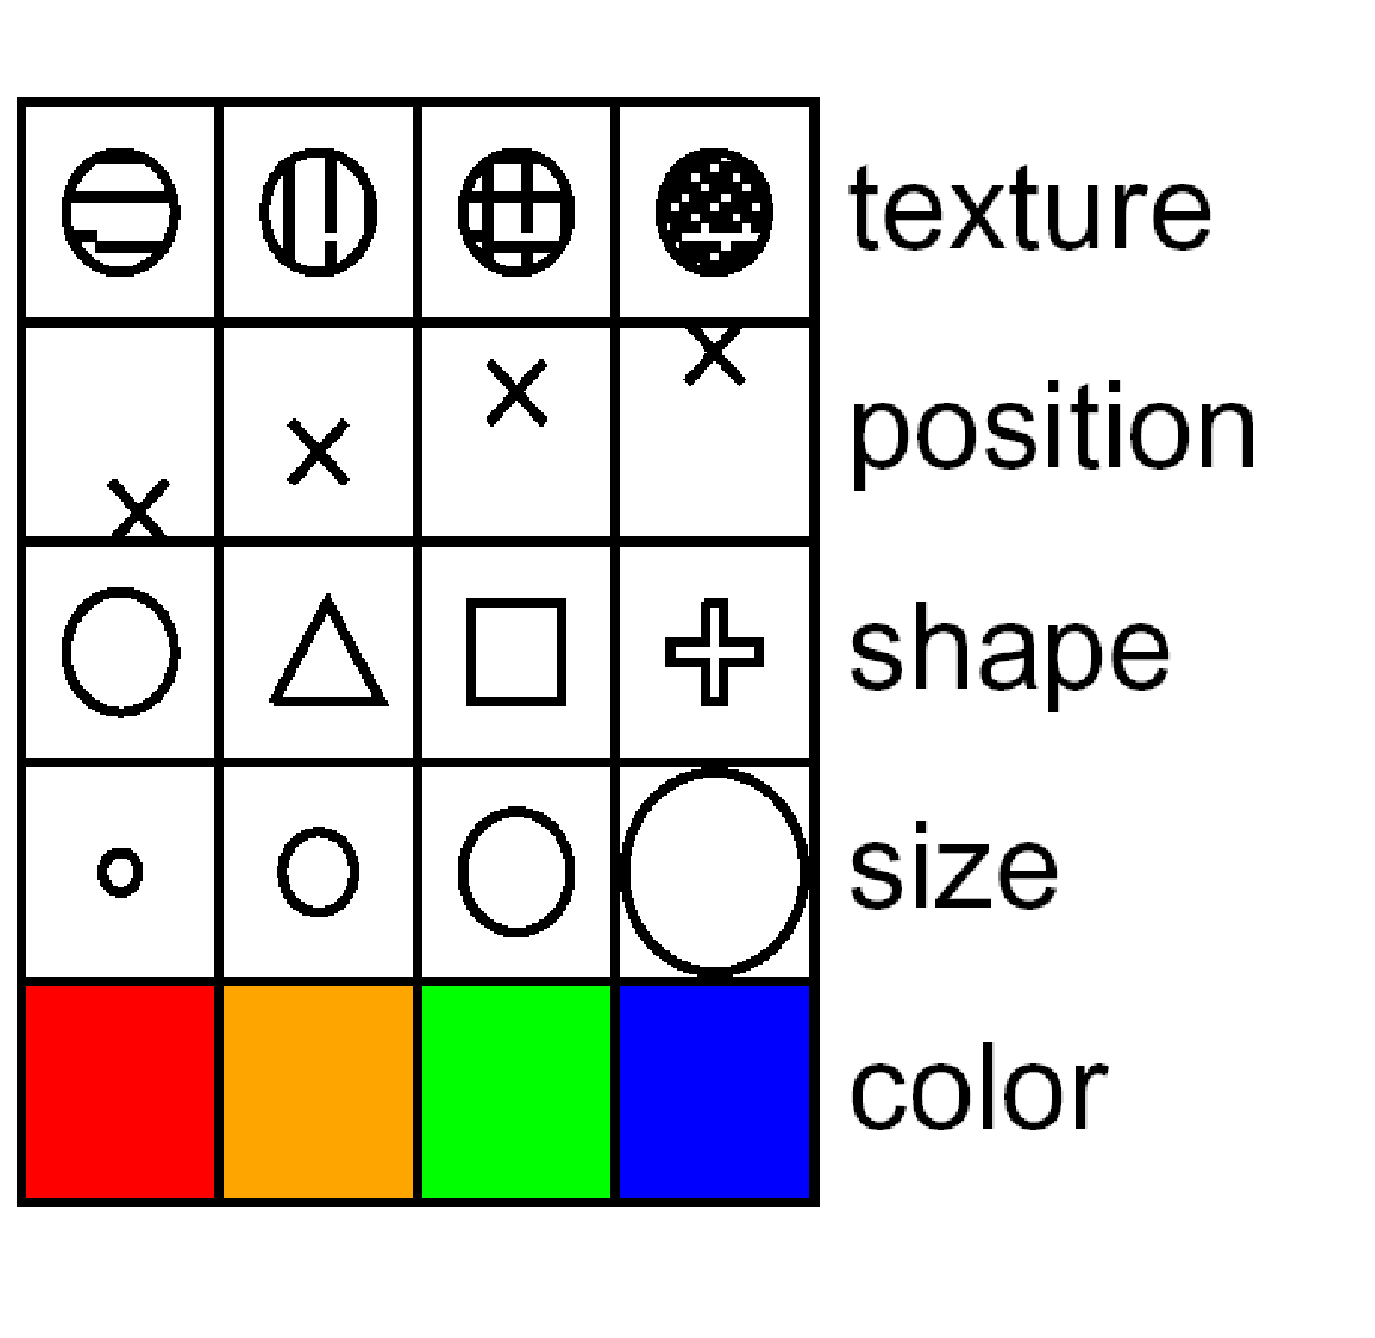
\includegraphics[width=42mm, height=35mm]{figures/xt_stim_layer2.eps}
%\end{center}
%\caption{Stimulus Input Layer: Caricature of input to the XT model, with rows portraying stimulus dimension (color, shape, size, etc) and columns indexing feature values across dimensions (small, medium, large, etc.)}
%\label{stimuluslayer-figure}
%\end{figure} 

The architecture of the XT model is shown in Figure~\ref{xt-layout-figure}.  This computational cognitive model makes use of the biologically grounded Leabra framework~\cite{OReillyRC:2000:Computational}.  The input of XT consists of two layers of neural units that can be used to specify the presentation of up to two stimulus objects.  It is natural to think of the rows of each input layer as representing different dimensions (e.g., color, shape, texture) and the columns indexing features across each dimension (e.g., red, orange, green, blue).  The Response layer has essentially the same structure as an input layer, with strong lateral inhibition among response units allowing the network to output a single stimulus feature (e.g., red) at a time.  The Response layer includes one additional unit, which codes for ``no response''.  

\begin{figure}
\begin{center}
	\includegraphics[width=125mm]{figures/xt_arch_2.ps}
\end{center}
\caption{XT Model Architecture.  The upper left corner shows a
         caricature of the input to the XT network, with rows
         portraying stimulus dimension (color, shape, size, etc.) and
         columns indexing feature values across dimensions (small,
         medium, large, etc.).  Each small box in this network diagram represents a Leabra processing unit, and arrows between layers represent complete unit-to-unit connectivity between layers.  The AG unit implements ``adaptive gating'' by modeling the effects of the dopamine system on PFC.}
\label{xt-layout-figure}
\end{figure} 

A collection of Hidden layers model posterior cortical circuits that
map from stimuli to responses.  Activity in these layers can be
adjusted, however, through top-down biasing signals from an actively
maintained representation in the PFC layer.  Unlike previous models,
the representations that can be maintained in PFC are learned through
a ``childhood development'' process that involves extensive training
on the performance of a variety of related tasks.  These developmental tasks
share a need to selectively attend to individual dimensions of the
stimuli.  For instance, the network might be presented with a large
red ball and a small red duck, and might be asked to identify the
feature that is the ``same'' across these two stimuli.  In this case,
the network must focus upon the ``color'' dimension and respond
``red''.  On each trial, corrective feedback is provided to drive
Leabra's synaptic learning processes, and correct responses from the
network produce an external reward signal ($r(t)$) of one (as opposed
to the usual zero reward).  Over time, the developmental training of
the network allows it to identify the separate dimensions of stimuli,
and it causes the network to hone its skill at focusing attention on a
single dimension at a time~\cite{RougierNP:2005:XT}.

The Task input to the network indicates which task is to be performed (e.g. the ``Naming Feature'' task, the ``Matching Feature'' task, the ``Smaller Feature'' task, or the ``Larger Feature'' task),
with one input unit coding for each task.  The Dimension Cue layer is
used to inform the network of the currently relevant stimulus
dimension.  For example, the Dimension Cue input is used to model the
Stroop task by informing the network when it should attend to the
color of the stimulus rather than its word form, or vice versa.  Each
unit in the Dimension Cue layer corresponds to a stimulus dimension,
and all of these inputs are turned off for tasks in which the network
must discover the relevant stimulus dimension on its own, as in WCST.

The flexible adjustment of cognitive control is implemented using a
DA-based adaptive gating (AG) mechanism.  The synaptic weights feeding
the special AG unit calculate an estimate of $V(t)$, and these weights
are adjusted based on $\delta(t)$ using a neural implementation of the
TD learning algorithm.  Importantly, the TD error, which encodes a DA
signal, is also used to manipulate the ``gate'' on the PFC layer.
When the model performs better than expected ($\delta(t) > 0$) the
current PFC representation is strengthened using an intrinsic
maintenance current to stabilize the existing pattern of activity.
When the model performs worse than expected ($\delta(t) < 0$), the
current PFC representation is destabilized, allowing a new, possibly
more appropriate PFC representation, based on the inputs into the PFC
layer, to be entertained.  In the model, the \begin{math}\delta(t)\end{math} value directly modulates excitatory ionic maintenance currents (\begin{math}g_m\end{math} below).  Large maintenance currents drive the membrane potential of simulated neurons in the PFC up, pushing them towards their maximal firing rate.  These currents are not allowed to become negative, being clipped at zero instead.  The maintenance currents, $g_m$, of simulated neurons in PFC are computed by:

\begin{equation}g_m(t-1) = 0 ~if~ |\delta(t)| > \theta\end{equation}
\begin{equation}g_m(t)_j = g_m(t-1) + \delta(t) a_j\end{equation}
\begin{center}$where~a_j~is~the~current~activation~value~of~PFC~unit~j$\end{center}

Therefore, a positive \begin{math}\delta(t)\end{math} will result in an increase in active maintenance of PFC representations, while a negative \begin{math}\delta(t)\end{math} will destabilize PFC.  The value \begin{math}\theta\end{math} represents a threshold value for the ionic currents.  If the TD error, \begin{math}\delta(t)\end{math}, exceeds this amount (\begin{math}\theta = .5\end{math} in all simulations), then the maintenance currents, \begin{math}g_m\end{math}, are effectively reset.  Over time, the network learns to maintain PFC representations that are likely to result in reward.  


XT is the first computational cognitive neuroscience model to explore
the development of PFC representations, and it is the first to provide
good quantitative fits to both Stroop and WCST data, for both
neurologically intact and frontally damaged people, based on a biologically informed architecture.

%\subsection{Modeling Autism Using XT}

%\subsubsection{General Approach}
%Based on the XT framework, my theory suggests that a deficit in DA functioning can account for the impaired cognitive flexibility seen in people with autism while leaving cognitive control robust and relatively unaffected.  We have tested this theory by reducing the effect of the DA signal in the XT model by scaling the TD error by a constant factor, $\kappa$, where $\kappa = 1$ for healthy individuals and $\kappa < 1$ for people with autism.  The scaling of $\delta(t)$ by $\kappa$ is the only modification from the original XT model that we have made in these simulations.  A $\kappa$ value of $0.54$ was found to produce the best fit to human performance, so this value was used in all of my simulations.  This reduction of the DA signal can be seen as decreasing the efficacy of the PFC gating system, resulting in the less efficient destabilization of PFC when errors are unexpectedly made.  The scaling was only used to modulate the simulated maintenance currents within the PFC layer, and not used to modify the learning of the weights into the Adaptive Gating unit.  An important point of future work is to also test the effects of this manipulation on these weights, weakening the overall influence that dopamine has on learning within circuits involved in the computation of future expected reward, as well.  

%It is worth noting that the modeled DA signal remains agnostic as to the precise quantitative nature of actual DA levels.  It is possible, for instance, that a optimal firing rate of the midbrain DA neurons exists for efficient PFC gating.  This implies \emph{either} too much or too little DA could have deleterious results on the effectiveness (a lower $\kappa$ value) of the DA based PFC gating system.

\subsection{Modeling WCST} 

%The WCST consists of a deck of cards, which contain stimuli varying along three dimensions (e.g., color, shape, quantity) and across four different features per dimension (e.g., for color dimension: red, orange, green, \& blue).  Participants are told to sort the cards into piles, but they are not given any instructions concerning how to do this correctly.  Instead, only sparse feedback ---``Correct'' or ``Incorrect''--- is given upon the placement of each card, until the proper sorting strategy is discovered.  After the sorting rule (e.g., sort by color) is learned by the participant, and $10$ consecutive correct sorts are accomplished, the rule is changed without informing the subject.  This procedure repeats until either $6$ correct categories (sets of $10$ correct consecutive sorts) are achieved, or all $127$ cards in the deck are exhausted.  Errors are recorded as incorrect sorts, with perseverative errors scored as an incorrect sort that used the last correct sorting rule.  Success at WCST requires the ability to flexibly change the dimension being maintained by PFC as the sorting rules change.  Modeling WCST in the XT framework required use of only three of the five possible input dimensions.  The same methods for administrating WCST to human participants were used in these simulations.

\begin{figure}
  \begin{center}
  \resizebox{8cm}{!}{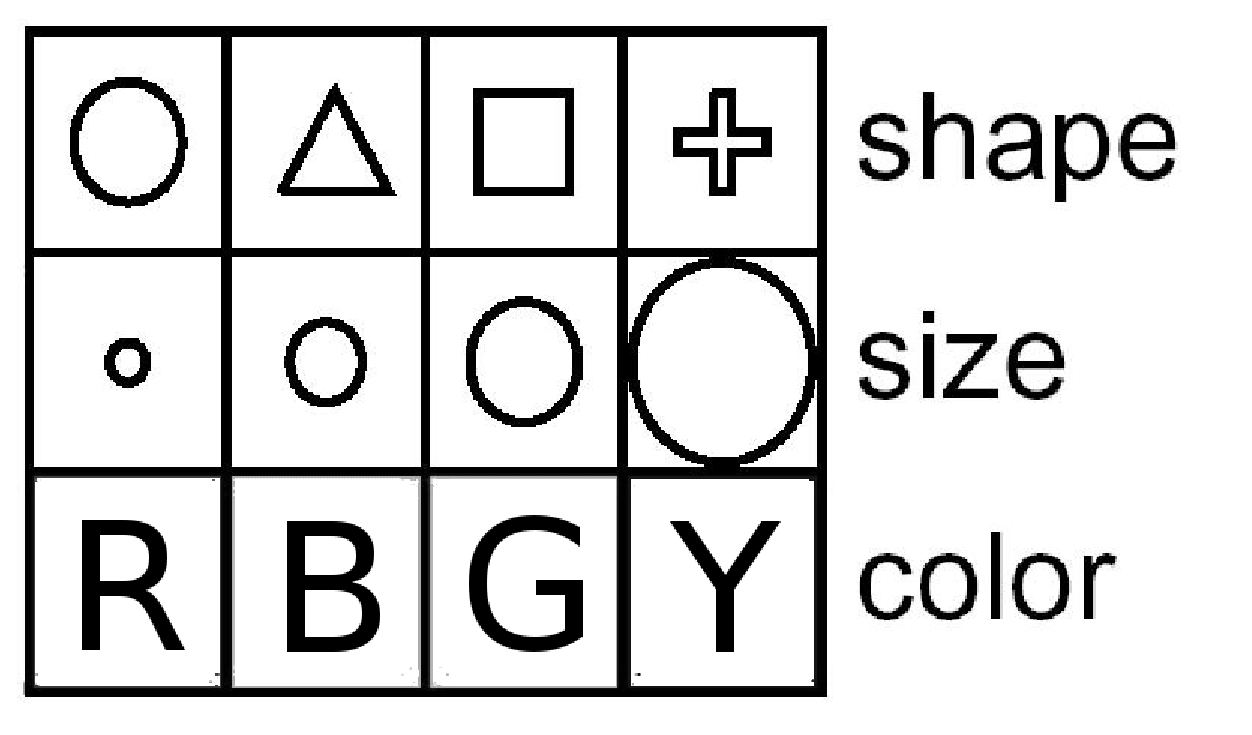
\includegraphics{figures/xt_wcst_stim}}
  \end{center}
  \caption{XT WCST example stimulus input}
  \label{xt_wcst_stim}
\end{figure}

In order to model the WCST the network was presented with stimuli at the input or ``stimulus array'' layer by activating individual units, one for a single feature across each of three dimensions.~(See Figure~\ref{xt_wcst_stim}.)  This input represented the current card to be sorted.  The task of the network was to name the currently relevant feature (e.g., the feature ``red'' if color is the currently relevant sorting dimension).  No information is provided via the Dimension Cue layer concerning which dimension should be used as the currently correct sorting rule, leaving the network to use a more-or-less random search strategy until the correct rule is discovered.  The network receives sparse feedback --- ``reward'' or ``no reward'' based on performance.  Left to only the random search strategy, the network's performance would tend towards chance.  However, XT is able to leverage the DA based AG mechanism coupled with the active maintenance and top-down influencing properties of the PFC layer in order to successfully perform the task.  The AG mechanism strengthens the PFC's intrinsic ionic maintenance currents when the network is performing well, allowing PFC to actively maintain currently relevant information.  The actively maintained PFC representations form a ``memory'' of the rule.  When the rule switches, the actively maintained representation becomes invalid.  If the network allows the invalid representation to influence subsequent processing, a large amount of perseverative errors will result.  The AG prevents this by providing a gating signal to PFC when reward is expected but not delivered, allowing a new representation to be acquired by PFC.


%Four main measures were used in evaluating the performance on the WCST task:

%	1. Total Number of Errors
%
%	2. Percentage of Total Errors 
%
%	3. Total Number of Perseverative Errors
%
%	4. Percentage of Perseverative Errors

%In the XT framework, the Dimension Cue layer is used to inform the network what dimension is currently relevant.  By *not* using this cue, the network is left to figure out what the sorting rule is by feedback alone, analogous to participants in WCST.  Only three of five possible dimensions where used in the stimulus layer in order to facilitate a tighter link with the model to that of the actual WCST task.  

\subsection{Modeling Stroop} 

%Stroop tests cognitive control by measuring the ability to inhibit a prepotent response.  In Stroop, the stimuli are different words presented in various colored fonts.  Participants are asked to either read the word or to name the color of the font in which the text is presented.  People are faster overall at reading the word as opposed to naming the color of the word.  Furthermore, when comparing the neutral (e.g., the word ``house'' in red font) versus the incongruent (e.g., the word ``green'' written in red font) conditions, people are slower in the incongruent case for color naming, but not for word reading.  This is known as Stroop interference.

%Cohen and Servan-Schreiber~(1990)\nocite{CohenJD:1990:Stroop} provided a computational account of the Stroop task. This model incorporated multiple associative pathways from stimulus features to possible responses.  They used a stronger, more automatic word reading pathway through posterior cortex and a relatively weak color naming pathway.  In their model, a task representation, maintained in PFC, provided top-down biasing, injecting extra activity into the color naming pathway when doing so was necessary to overcome the prepotent word reading pathway (i.e., when asked to name the font color).  The resulting competition between the two strong pathways resulted in an increase in response time in the color naming incongruent condition.  Response time was not increased in the word reading incongruent condition, however, as the weaker color naming pathway, when unsupported by PFC, offered little competition.

The XT model addresses the Stroop task in much the same way as Cohen and Servan-Schreibers seminal model on the Stroop task~\cite{CohenJD:1990:Stroop}.  Specifically by leveraging competition between pathways with different levels of strength or prepotency, the stronger word reading pathway and the weaker color namingi pathway.  In order to simulate the relative prepotency of a stimulus dimension in my model, we manipulated the frequency in which one dimension (font color) was experienced during training, making the dimension relevant only 25\% as often as the other dimensions (word reading).  
%The settling time, in ``cycles'', of the network was linearly scaled to ``milliseconds'' using a single free parameter, allowing a direct comparison between model results and human data.

\subsection{Model Simulation Results}

\subsubsection{Simulations} 
A total of $100$ networks were prepared using the XT developmental
training procedure, stopping when the network achieved a stringent
performance criterion, or after a maximum of $100$ epochs.  Each
network was then tested under both conditions of DA modulation ($\kappa = 1$ for healthy networks and $\kappa = .54$ for modeled autistic performance), on
each of the WCST and the Stroop tasks.  The $100$ networks were each
treated as individual subjects for the purposes of data analysis.

\subsubsection{WCST Results} 
WCST simulations of both healthy individuals ($\kappa = 1$) and persons with autism ($\kappa = 0.54$) 
provided results matching those reported in the literature.  The differences between the 
simulated performance of normally functioning individuals and the
simulated autistic performance were statistically reliable
($p < 0.001$), and consistent with previous
studies~\cite{PriorMR:1990:AutismWCST,Ozonoff:1999:AutismStroopWCST,MinshewNJ:2002:AutismWCST}.
In particular, the perseverative error measure was significantly
higher in the DA modulated version of my model as compared to the
model of normal function.  (See Figure~\ref{wcst-figure}.)


\begin{figure}
\begin{center}
	\includegraphics[width=110mm]{graphs/wcst.ps}
                                                                
\textcolor{white}{\\--------------------------------\\}

	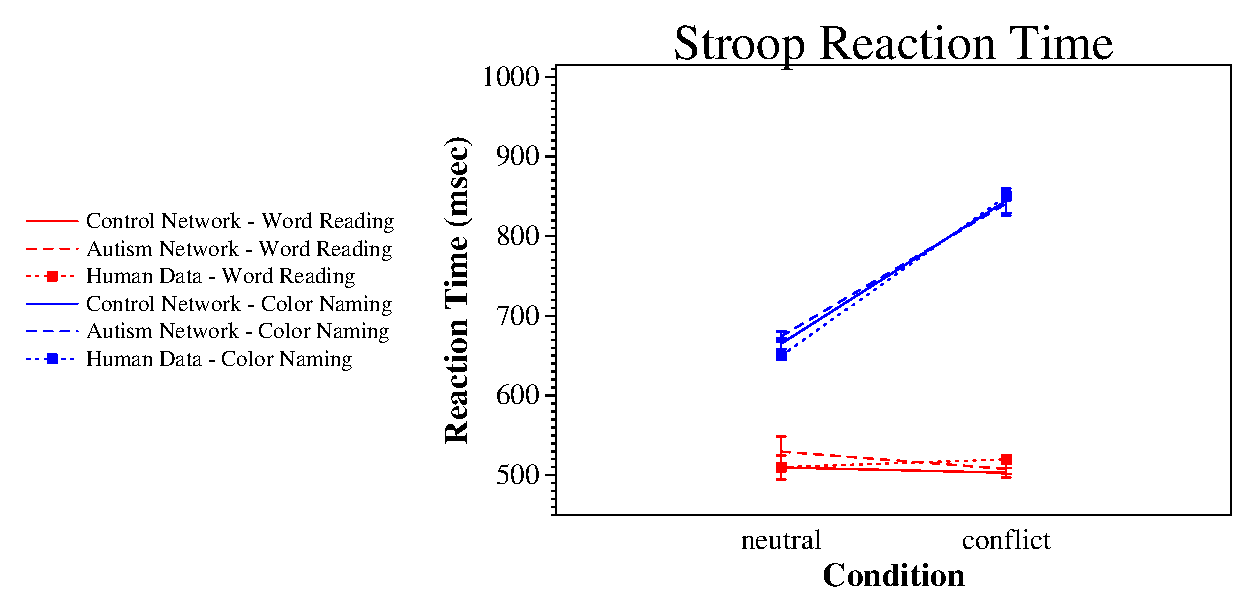
\includegraphics[width=110mm]{graphs/stroop.ps}
\end{center}
\caption{Top: Comparing model performance on WCST perseveratitive errors for normally functioning and individuals with autism to a previous study (Minshew et al., 2002). Model results capture performance of people with autism, committing significantly more perseverative errors. Error bars are standard errors of the mean.  Bottom: Stroop reaction time plot comparing the simulated autistic and normally functioning network's performance to human data. Healthy human data from~Dunbar et al. (1984).  Autistic subjects perform no differently than controls~(Ozonoff et al., 1999).  Error bars are standard errors of the mean.} 
\label{wcst-figure}
\end{figure} 

\subsubsection{Stroop Results} 

Model performance on the Stroop task provided a good quantitative fit to human performance.  (See Figure~\ref{wcst-figure}.) The model with intact DA function displayed the classic Stroop reaction time results.  The prepotent word reading dimension showed uniform reaction times across both congruent and conflict conditions, while the weaker color naming dimension exhibited a slowing in reaction times when the stimuli were incongruent.  The performance of the autistic model was virtually identical, with no significant increase in the overall Stroop effect ($F(1,198) = 0.62$; $p > 0.43$), which is consistent with past findings~\cite{Ozonoff:1999:AutismStroopWCST}.


\subsubsection{Developmental Results}

The initial simulations involved the introduction of a DA deficit only
after the model was fully developed.  Thus, these simulations ignored
the possibility that an early manifestation of a DA deficit might
hinder the proper learning of PFC representations, introducing an
impairment in cognitive control in the model that is not observed in
autistic subjects.  A second set of simulations was conducted to
address this issue and to examine the developmental time course of
cognitive control and cognitive flexibility in these models.  PFC
development and model performance were analyzed over the entire
developmental period of the model ($100$ epochs).  Two groups of $10$
networks (individuals) were used: an autistic group with $\kappa = 0.54$
and a control group with $\kappa = 1.00$.  At the end of developmental
training, the networks exhibited the same pattern of results as seen
in the initial simulations.  Furthermore, the developmental time
course data provided some insight into why executive deficits might
appear late in autism, as described in the
literature~\cite{GriffithEM:1999:AutismYoungED}.  This insight can be had by carefully examining how PFC representations change in the model over time, and how these representations affect Stroop and WCST performance.

\subsubsection{PFC Representations} 

Figures~\ref{rep1-figure} and \ref{rep2-figure} plot the synaptic
strengths from the PFC layer to the Response layer.  Each large box
corresponds to a PFC unit, and each encapsulated small box corresponds
to a Response unit, with the strength of the connection from the given
PFC unit to the given Response unit being reflected in the brightness
of the box (lighter means stronger).  Note that each row designates
connections to Response layer units representing features in the same
stimulus dimension.  (See the upper left corner of
Figure~\ref{xt-layout-figure}.)  Thus, these plots can be used to
examine the degree to which the PFC layer developed a representational scheme that allowed for the selective modulation of individual stimulus dimensions.  For a given PFC unit (large box), a bright row of connections (small boxes) indicates that that unit selectively supports attention to the stimulus dimension corresponding to that row.  In
Figure~\ref{rep1-figure}, which was generated early in developmental
training, both the autistic network and the control network lack
strong dimensional weights.  However, in Figure~\ref{rep2-figure},
both networks have developed strong dimensional representations in
PFC, as evidenced by the extremely salient horizontal bands of
``strong'' weights.  Thus, appropriate PFC representations were
acquired only slowly over the course of developmental training, and
the DA manipulation did not hinder the formation of these
representations.

\begin{figure}[t]
\begin{center}
	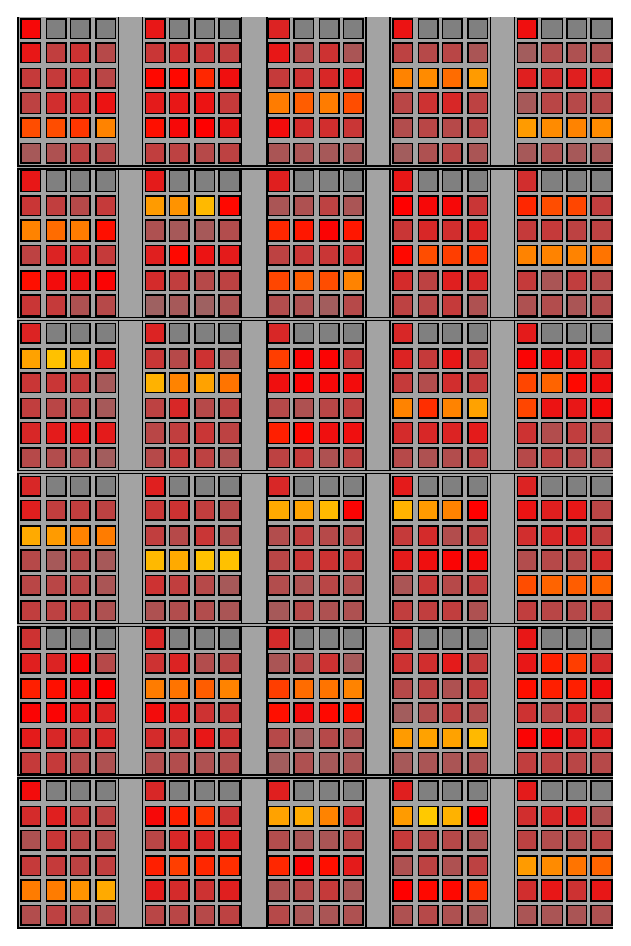
\includegraphics[width=35mm,height=55mm]{graphs/PFCwts1.05.eps}
	\hspace{18 mm}
	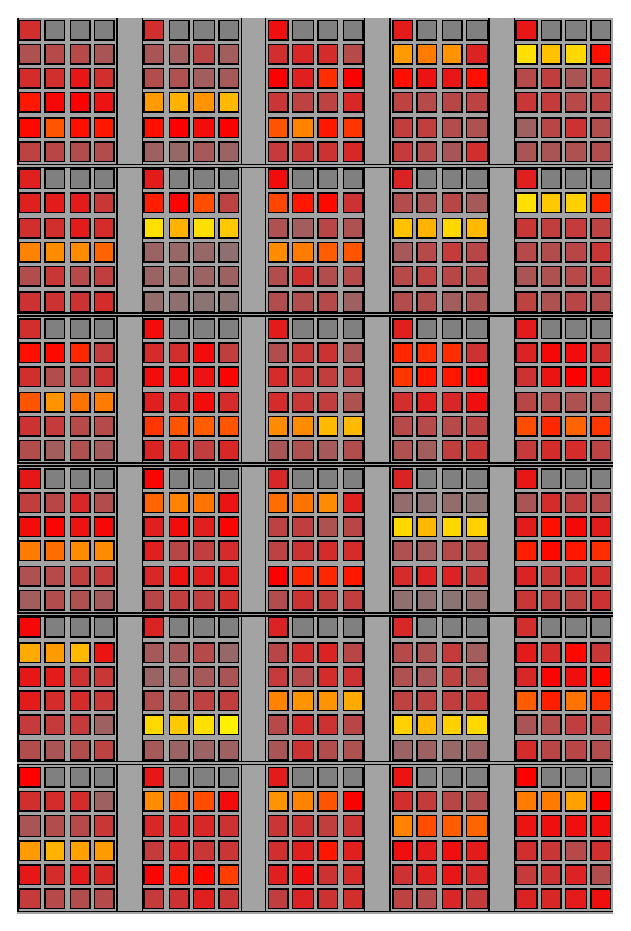
\includegraphics[width=35mm,height=55mm]{graphs/PFCwts54.05.eps}
\end{center}
\caption{PFC Representations early in development
         (epoch 5): left - control model, right -
         autism model.  Each large box corresponds to the connection strength from that PFC unit, and each small box corresponds to the connection strength from that PFC unit to a Response layer unit, with strength growing with brightness.  Note the lack of any strong dimensional representations in both versions.}
\label{rep1-figure}
\end{figure} 

\begin{figure}[th]
\begin{center}
	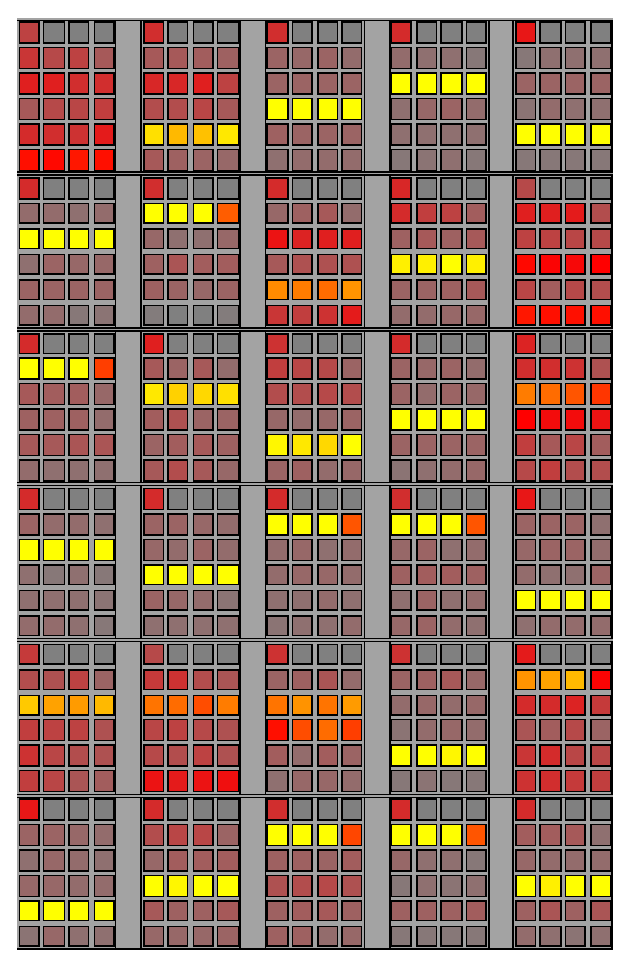
\includegraphics[width=35mm,height=55mm]{graphs/PFCwts1.100.eps}
	\hspace{18 mm}
	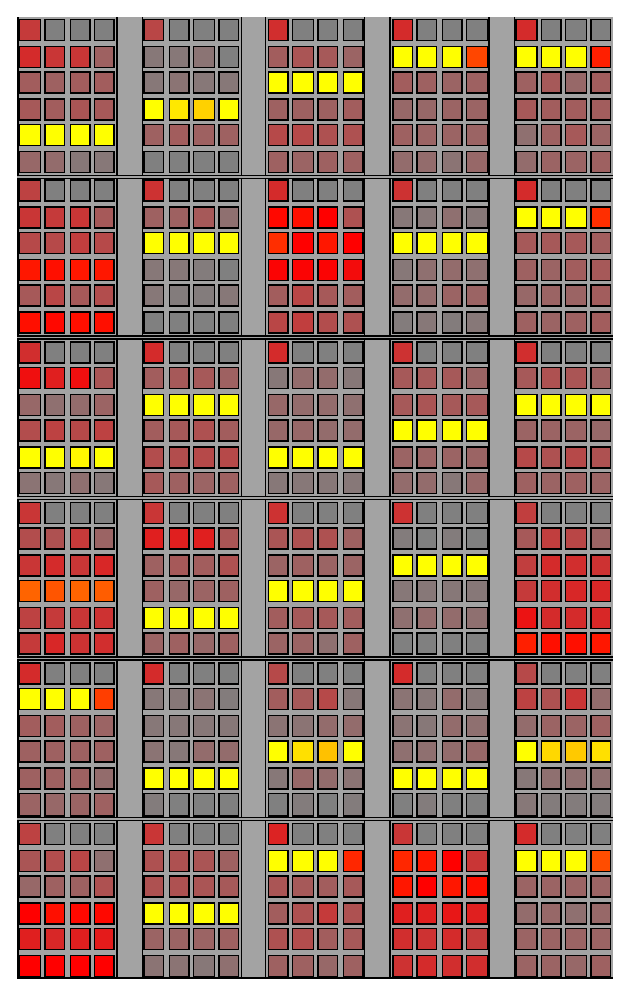
\includegraphics[width=35mm,height=55mm]{graphs/PFCwts54.100.eps}
\end{center}
\caption{PFC Representations late in development
         (epoch 100): left - control model, right -
         autism model.  Each large box corresponds to the connection strength from that PFC unit, and each small box corresponds to the connection strength from that PFC unit to a Response layer unit, with strength growing with brightness.  Strong dimensional representations have formed
         in both models, as exhibited by strong weights from individual PFC units to all of the Response layer features for a given dimension.}  
\label{rep2-figure}
\end{figure} 


\subsubsection{Executive Dysfunction Development} 

Introducing a deficit in the DA-based gating mechanism from the
beginning of development still allows the network to capture autistic
performance on tasks requiring cognitive flexibility and control.  In
Figures~\ref{stroop-devel-figure} \& \ref{wcst-devel-figure}, the
Stroop interference effect and the number of perseverative errors in
WCST are plotted as a function of developmental training time.
Figure~\ref{stroop-devel-figure} shows no effect of the
DA-manipulation across development.  Stroop interference was
significantly greater for the autistic networks during only $1$ training epoch
out of the $100$ ($p<.003$), demonstrating robust cognitive control
throughout the entirety of development.
Figure~\ref{wcst-devel-figure}, however, demonstrates a significant
increase in the number of perseverative errors made by the
DA-modulated network as early as epoch $12$.  During the first $53$
epochs there was a significant difference ($p < 0.05$) during only
$26.4\%$ of the epochs.  However, later in the development of the
model (epochs $54-100$) a significant difference was reached $93.6\%$
of the time.  Interestingly, neither ``healthy'' models nor
DA-deficient models showed a distinct advantage or disadvantage during
the earliest stages of development.  We believe that the lack of
executive deficits early in the development of these models was
largely due to the fact that both models lacked strong PFC
representations early in training.  Without strong, dimensional PFC
representations, the models were forced to rely more heavily on the
Hidden layers (posterior cortex) to perform the tasks.  Since
weakening the DA-based gating mechanism had no effect on these
``posterior'' areas of the model, neither model showed any advantage
over the other at this early stage.

\subsection{Summary}

Given the XT account of the role of PFC in executive control, we have shown that a single manipulation --- reducing the efficacy of the DA signal --- is sufficient to capture the pattern of performance exhibited by people with autism on basic tests of cognitive flexibility (WCST) and cognitive control (Stroop).  Furthermore, we demonstrated that weakening the DA-based gating mechanism over the entire course of PFC development continues to reflect both the ``strengths'' and ``weaknesses'' of autistic performance, while also providing some insight into the late appearance of cognitive flexibility deficits in autism.  Specifically, the absence of strong PFC representations early in development masks the problematic PFC/DA interactions.  Early in development, both normally developing and autistic individuals face these tasks without much useful support from PFC, so the PFC gating mechanism matters little.  As the model continues to develop, however, and the PFC representations strengthen, the weakened DA based gating mechanism manifests itself behaviorally as impaired cognitive flexibility.

\begin{figure}[t]
\begin{center}
	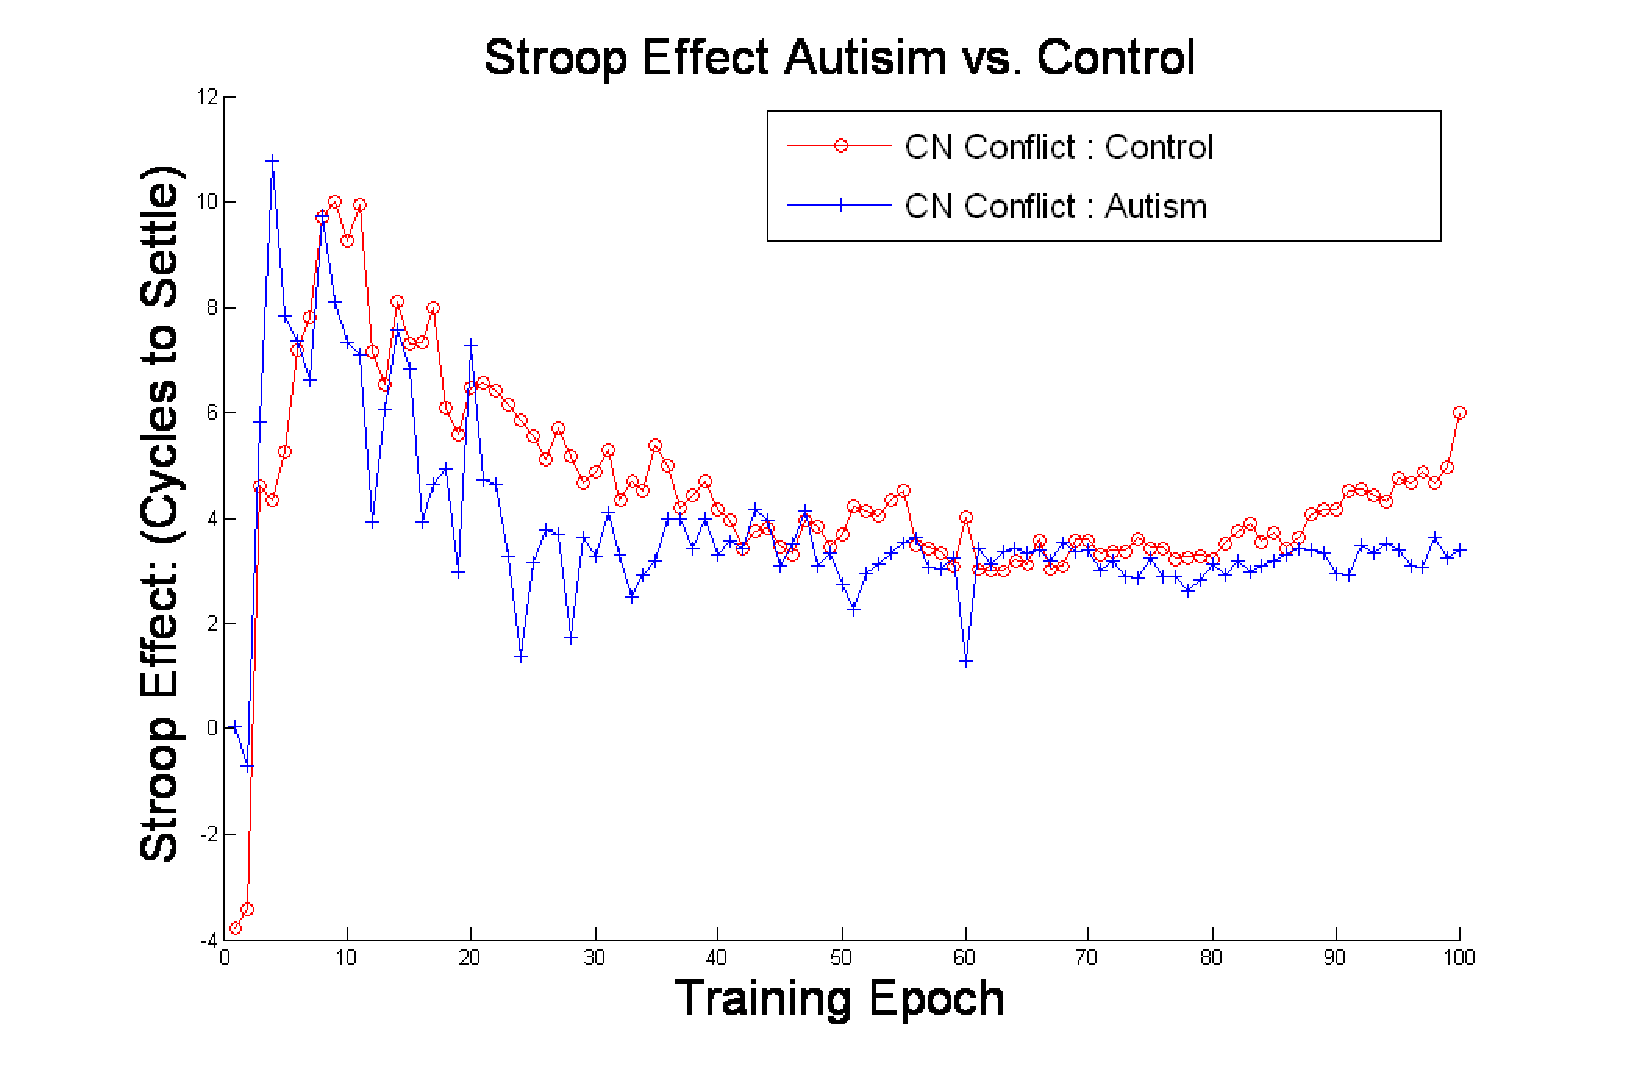
\includegraphics[width=145mm]{graphs/stroop_devel.eps}
\end{center}
\caption{Stroop interference score for the model over the course of development.} 
\label{stroop-devel-figure}
\end{figure} 

\begin{figure}[t]
\begin{center}
	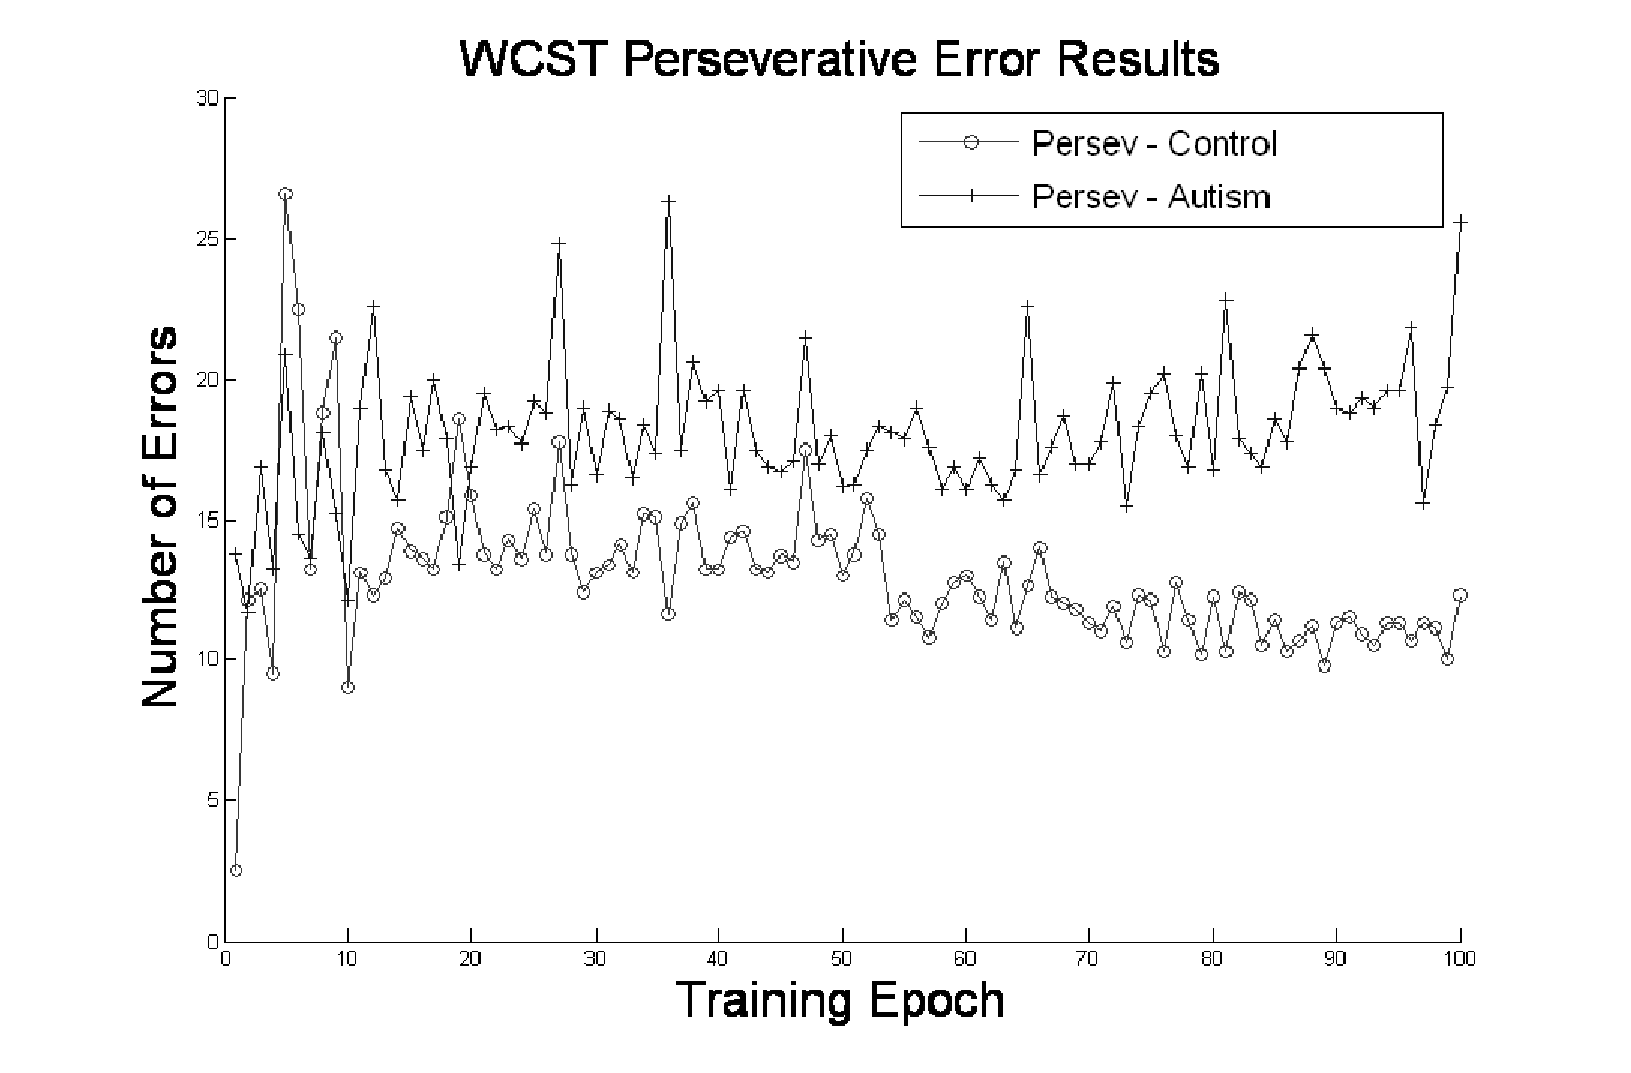
\includegraphics[width=145mm]{graphs/wcst_devel_persev.eps}
\end{center}
\caption{WCST perseverative error count for the model over the course of developmental training.} 
\label{wcst-devel-figure}
\end{figure} 

